\documentclass[11pt]{article}
\usepackage[margin=1in]{geometry}
\usepackage{graphicx}
\usepackage{amsmath}
\usepackage{float}
\usepackage[hidelinks]{hyperref}
\usepackage{enumitem}
\usepackage{booktabs}
\usepackage{xcolor}
\usepackage{listings}

\lstdefinestyle{matlabstyle}{
    language=Matlab,
    basicstyle=\ttfamily\small,
    breaklines=true,
    columns=fullflexible,
    frame=single,
    keepspaces=true,
    showstringspaces=false,
    keywordstyle=\color{blue},
    commentstyle=\color{teal!70!black},
    stringstyle=\color{orange!60!black}
}

\lstset{style=matlabstyle}

\begin{document}

\begin{center}
{\LARGE ME 656: Autonomous Navigation for Mobile Robots}\\[0.5em]
{\Large Simulation Lab 2 Report}\\[1em]
\begin{tabular}{ll}
Course: & ME 656 - Autonomous Navigation for Mobile Robots \\
Semester: & Spring 2026 \\
Assignment: & SimLab 2 \\
Student: & Matthew Lepis \\
\end{tabular}
\end{center}

\vspace{1em}

\section{Overview}
This report summarizes the path-planning and localization-uncertainty results
for Simulation Lab 2. The robot was planned through the provided 2D obstacle
workspace using a Rapidly-exploring Random Tree (RRT). For each generated path,
a linear Kalman filter covariance propagation was used to estimate the expected
localization uncertainty along the path.

One representative run used 1000 RRT trials. From those trials, four paths
were selected: the shortest path, the minimum terminal uncertainty path, the
maximum terminal uncertainty path, and a best-tradeoff path. The best-tradeoff
path was selected using a normalized cost function with equal weighting between
path length and terminal uncertainty. A second run using 100,000 RRT trials was
also generated to examine how the quality of the selected paths improves as
the number of randomized planning attempts increases.

\section{Implementation Details}

The main driver script, \texttt{simlab2.m}, coordinates the full simulation.
First, \texttt{simulation\_configuation.m} builds a configuration struct that
contains the workspace, start state, goal region, obstacle list, RRT
parameters, sensor range, Kalman filter time step, plotting options, and
best-path scoring weights. The driver then calls \texttt{RRT.m} to generate a
cell array of randomized RRT trials. Each trial stores the recovered path and
the total path length.

\subsection{RRT Path Generation}
The RRT implementation is organized around two classes: \texttt{Tree.m} and
\texttt{TreeNode.m}. A \texttt{TreeNode} stores the 2D state, its parent and
children, the edge cost from its parent, and the action used to reach it. The
\texttt{Tree} object stores the list of vertices and the simulation
configuration. During each RRT expansion, the tree samples a random state
within the workspace bounds, finds the nearest existing tree node, and attempts
to grow toward the sample by the fixed growth distance of 2 m.

Before a new node is accepted, the code checks both the candidate point and the
line segment from the nearest node to the candidate node. The helper function
\texttt{collision\_check\_point.m} rejects candidate states that fall inside an
obstacle, while \texttt{collision\_check\_segment.m} rejects edges that
intersect obstacle boundaries. The tree continues expanding until a new node
lands inside the goal region. Once this occurs, \texttt{RRT.m} reconstructs the
solution path by following parent pointers from the goal node back to the root
and summing the edge costs to obtain the path length.

\subsection{Measurement Visibility and Kalman Covariance Propagation}
After all RRT trials are generated, the driver propagates the Kalman filter
covariance along every path using \texttt{propagate\_KF\_path.m}. This function
first converts the selected RRT path into a lighter struct representation that
contains only the data needed for covariance propagation. It then calls
\texttt{collect\_sensor\_data.m} to determine which position measurements are
available at each path node.

The sensing model follows the assignment description. The robot has four
axis-aligned range beams with range 5 m. If a horizontal beam intersects an
obstacle, the robot is treated as having an $x$-position measurement. If a
vertical beam intersects an obstacle, the robot is treated as having a
$y$-position measurement. Odometry measurements of velocity are always
available. Therefore, the measurement matrix $H_k$ changes size from node to
node depending on obstacle visibility.

For covariance propagation, the state is
\[
    x_k = [x\;\; y\;\; \dot{x}\;\; \dot{y}]^T.
\]
The code uses a constant-velocity transition matrix with $\Delta t = 1$ s,
process noise covariance $Q=I$, initial covariance $P_0=I$, and measurement
noise covariance $R_k=I$ with dimension matched to the available measurements.
At each node, the predicted covariance is computed as
\[
    P_{k|k-1} = A P_{k-1} A^T + Q,
\]
and the posterior covariance is updated using the information-form expression
\[
    P_k =
    \left(P_{k|k-1}^{-1} + H_k^T R_k^{-1} H_k\right)^{-1}.
\]
The scalar terminal uncertainty for each path is then computed as
\[
    \mathrm{tr}(P_{\mathrm{final}}).
\]

\subsection{Path Selection and Plotting}
Once every trial has a terminal covariance trace, the driver selects several
representative paths. The shortest path is selected by
\texttt{find\_shortest\_path.m}, while the minimum- and maximum-uncertainty
paths are selected directly from the terminal uncertainty array. The
best-tradeoff path is selected by \texttt{find\_best\_path.m}, which normalizes
path length and terminal uncertainty to comparable 0--1 ranges and computes
\[
    J = w_d \bar{d} + w_u \bar{u}.
\]
For the results shown here, the weights were set to $w_d=w_u=0.5$, giving
equal importance to path length and terminal uncertainty.

The plotting functions separate visualization from the planning logic.
\texttt{plot\_path.m} draws the selected path and labels its length and
terminal uncertainty. \texttt{plot\_covariance\_evolution.m} visualizes the
position covariance block $P(1\!:\!2,1\!:\!2)$ at each node. The eigenvectors of
this block determine the orientation of each ellipse, while the square roots of
the eigenvalues determine the one-standard-deviation major and minor axes.
The helper \texttt{selection\_color.m} keeps the path and ellipse colors
consistent for the shortest, minimum-uncertainty, maximum-uncertainty, and
best-tradeoff paths.

\section{Selected Paths}
\begin{table}[H]
\centering
\begin{tabular}{lccc}
\toprule
Path type & Trial & Path length (m) & Terminal uncertainty, $\mathrm{tr}(P)$ \\
\midrule
Shortest path & 193 & 100.00 & 47.42 \\
Minimum uncertainty & 442 & 108.00 & 9.56 \\
Maximum uncertainty & 752 & 130.00 & 251.39 \\
Best tradeoff & 811 & 103.10 & 13.55 \\
\bottomrule
\end{tabular}
\caption{Selected path outcomes from 1000 RRT trials.}
\label{tab:path-results}
\end{table}

\begin{figure}[H]
\centering
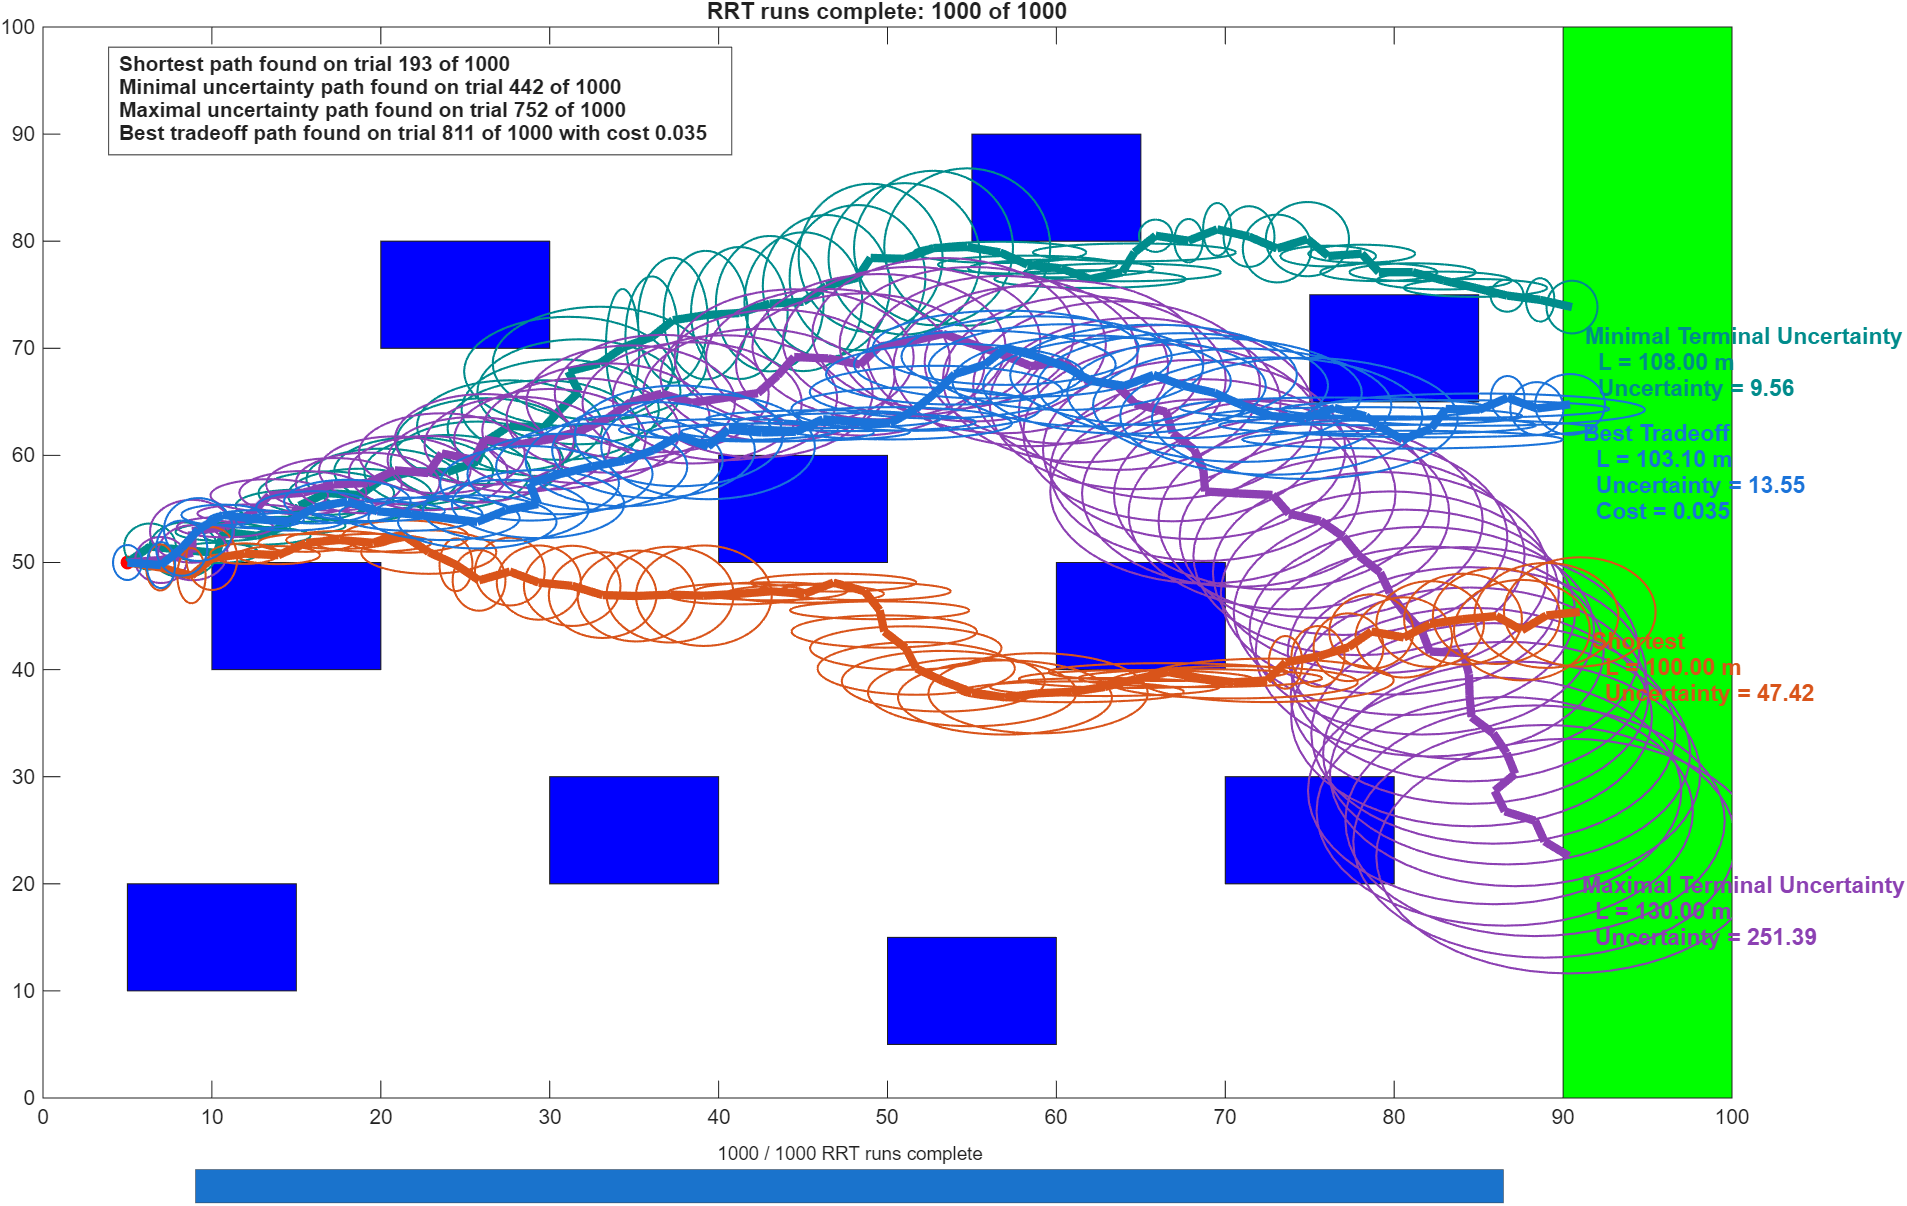
\includegraphics[width=0.95\textwidth]{Figure_2.png}
\caption{Selected RRT paths and Kalman filter covariance ellipses for the
1000-trial run.}
\label{fig:selected-paths}
\end{figure}

\begin{table}[H]
\centering
\begin{tabular}{lccc}
\toprule
Path type & Trial & Path length (m) & Terminal uncertainty, $\mathrm{tr}(P)$ \\
\midrule
Shortest path & 60875 & 96.61 & 63.27 \\
Minimum uncertainty & 54584 & 117.00 & 9.56 \\
Maximum uncertainty & 40468 & 140.00 & 283.98 \\
Best tradeoff & 58063 & 98.23 & 11.54 \\
\bottomrule
\end{tabular}
\caption{Selected path outcomes from 100,000 RRT trials.}
\label{tab:path-results-100000}
\end{table}

\begin{figure}[H]
\centering
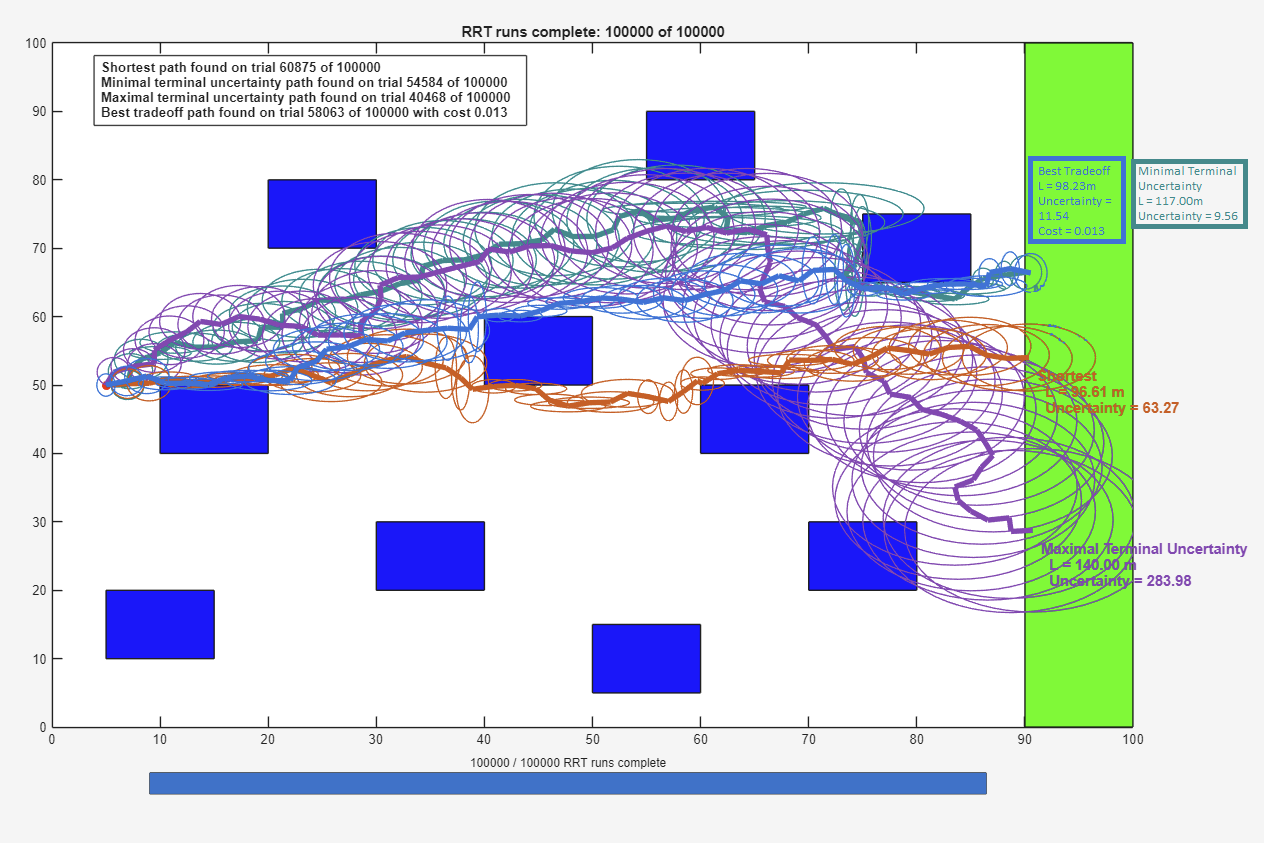
\includegraphics[width=0.95\textwidth]{Figure_3.png}
\caption{Selected RRT paths and Kalman filter covariance ellipses for the
100,000-trial run.}
\label{fig:selected-paths-100000}
\end{figure}

The shortest path is the most direct route to the goal. It moves nearly
horizontally across the workspace while avoiding obstacles along the way. This
keeps the total distance low at 100 m, but the terminal uncertainty is higher
than both the minimum-uncertainty and best-tradeoff paths. The shortest and
minimum-uncertainty paths pass comparably near obstacles, but they do so at
different points in the workspace.

The minimum-uncertainty path takes a longer route, with a path length of 108 m,
but ends with much lower terminal uncertainty. A key difference is that near
the end of its path, the robot observes an obstacle closer to the goal than it
does on the shortest path. This gives the Kalman filter additional position
information later in the trajectory, which reduces the final covariance.

The maximum-uncertainty path is both long and poorly localized. It appears to
spend the longest duration outside useful sensing range, especially toward the
end of the path. During these portions of the trajectory, process noise
continues to increase the covariance while there are few or no position
measurements to reduce it. As a result, this path reaches a terminal
uncertainty of 251.39.

The 100,000-trial result reinforces the same trend while producing a stronger
best-tradeoff path. In that run, the best-tradeoff path had a path length of
98.23 m and terminal uncertainty of 11.54. This path was only slightly longer
than the 96.61 m shortest path from the same run, but had much lower terminal
uncertainty than that shortest path. This illustrates the benefit of evaluating
many randomized RRT instances: the planner has more chances to discover paths
that are both short and informative for localization.

\section{Distance, Uncertainty, and Collision Risk}
Traveling near obstacles can improve localization because the robot can compare
range-beam observations against the known map. When an obstacle is visible from
a horizontal beam, the robot effectively gains information about its
$x$-position. When an obstacle is visible from a vertical beam, it gains
information about its $y$-position. These measurements reduce the corresponding
components of the error covariance matrix.

This same behavior also introduces collision risk. Because the robot has
nonzero localization uncertainty, the actual robot position may differ from the
nominal planned state. If a covariance ellipse intersects an obstacle, then
there is a plausible localization error under which the robot could be in
collision even though the nominal path is collision-free. Therefore, a good
path should not simply stay as close as possible to obstacles. It should use
obstacle visibility enough to reduce uncertainty while still maintaining
reasonable clearance.

Additional distance is worthwhile only when it produces a meaningful reduction
in uncertainty. A longer path that does not pass through informative sensing
regions can increase distance without improving localization. To capture this
tradeoff, the best-tradeoff path was selected using
\[
    J = w_d \bar{d} + w_u \bar{u},
\]
where $\bar{d}$ is normalized path length, $\bar{u}$ is normalized terminal
uncertainty, and $w_d = w_u = 0.5$ for this run. With equal weighting, the
best-tradeoff path had a path length of 103.1 m and terminal uncertainty of
13.55. This is slightly longer than the shortest path, but it substantially
reduces terminal uncertainty. It is also less certain than the
minimum-uncertainty path, but it achieves most of the uncertainty reduction
with less additional distance.

The most reasonable weighting depends on the application. A time-critical task
would place more weight on distance, while a precision navigation task would
place more weight on uncertainty. For this run, the equal-weighted
best-tradeoff path is a useful middle ground between minimizing travel distance
and minimizing terminal covariance.

\section{Number of RRT Trials}
Increasing the number of RRT trials improved the quality of the selected
paths. With more trials, the algorithm had more opportunities to sample paths
that were smoother, more direct, or more informative from a localization
standpoint. In this workspace, 1000 trials produced noticeably better paths
than 100 trials, and the 100,000-trial run produced an even stronger
best-tradeoff path.

Based on these results, 100 trials is useful but not reliably sufficient for
finding a high-quality path. More than 100 trials gives the selection process a
better set of candidate paths, especially when optimizing for both path length
and localization uncertainty. For this workspace, 1000 trials provided a more
reliable basis for identifying the shortest, minimum-uncertainty,
maximum-uncertainty, and best-tradeoff paths, while the 100,000-trial run
showed that still larger sample counts can continue to improve the selected
tradeoff path.

\section{Assumptions}
These observations are based on the SimLab 2 assumptions: the robot is modeled
as a point, the workspace obstacles are known and rectangular, the robot
follows the planned path exactly, and the Kalman filter is used to predict
covariance growth rather than to correct a simulated perturbed trajectory. The
results also depend on randomized RRT samples, so individual selected paths can
change from run to run.

\section{Included MATLAB Files}
The MATLAB source associated with this report is organized as follows:
\begin{itemize}[leftmargin=1.5em]
    \item \texttt{simlab2/simlab2.m}: driver script that runs the RRT trials,
    propagates covariance, selects representative paths, and plots results
    \item \texttt{simlab2/RRT.m}, \texttt{simlab2/Tree.m}, and
    \texttt{simlab2/TreeNode.m}: RRT implementation and tree data structures
    \item \texttt{simlab2/propagate\_KF\_path.m} and
    \texttt{simlab2/collect\_sensor\_data.m}: Kalman covariance propagation
    and obstacle-visibility measurement logic
    \item \texttt{simlab2/find\_shortest\_path.m} and
    \texttt{simlab2/find\_best\_path.m}: path-selection helpers
    \item \texttt{simlab2/plot\_path.m},
    \texttt{simlab2/plot\_covariance\_evolution.m}, and
    \texttt{simlab2/selection\_color.m}: plotting utilities for selected paths
    and covariance ellipses
    \item \texttt{simlab2/generate\_obstacles.m},
    \texttt{simlab2/collision\_check\_point.m},
    \texttt{simlab2/collision\_check\_segment.m}, and
    \texttt{simlab2/ellipse.m}: workspace, collision-checking, and ellipse
    helper functions
\end{itemize}

\appendix
\section{MATLAB Source Code}

\subsection*{\texttt{simlab2.m}}
\lstinputlisting[caption={\texttt{simlab2.m}}, label={lst:simlab2m}]{../simlab2.m}

\subsection*{\texttt{simulation\_configuation.m}}
\lstinputlisting[caption={\texttt{simulation\_configuation.m}}, label={lst:simulationconfiguation}]{../simulation_configuation.m}

\subsection*{\texttt{RRT.m}}
\lstinputlisting[caption={\texttt{RRT.m}}, label={lst:rrtm}]{../RRT.m}

\subsection*{\texttt{Tree.m}}
\lstinputlisting[caption={\texttt{Tree.m}}, label={lst:treem}]{../Tree.m}

\subsection*{\texttt{TreeNode.m}}
\lstinputlisting[caption={\texttt{TreeNode.m}}, label={lst:treenodem}]{../TreeNode.m}

\subsection*{\texttt{propagate\_KF\_path.m}}
\lstinputlisting[caption={\texttt{propagate\_KF\_path.m}}, label={lst:propagatekfpath}]{../propagate_KF_path.m}

\subsection*{\texttt{collect\_sensor\_data.m}}
\lstinputlisting[caption={\texttt{collect\_sensor\_data.m}}, label={lst:collectsensordata}]{../collect_sensor_data.m}

\subsection*{\texttt{find\_shortest\_path.m}}
\lstinputlisting[caption={\texttt{find\_shortest\_path.m}}, label={lst:findshortestpath}]{../find_shortest_path.m}

\subsection*{\texttt{find\_best\_path.m}}
\lstinputlisting[caption={\texttt{find\_best\_path.m}}, label={lst:findbestpath}]{../find_best_path.m}

\subsection*{\texttt{plot\_path.m}}
\lstinputlisting[caption={\texttt{plot\_path.m}}, label={lst:plotpath}]{../plot_path.m}

\subsection*{\texttt{plot\_covariance\_evolution.m}}
\lstinputlisting[caption={\texttt{plot\_covariance\_evolution.m}}, label={lst:plotcovarianceevolution}]{../plot_covariance_evolution.m}

\subsection*{\texttt{selection\_color.m}}
\lstinputlisting[caption={\texttt{selection\_color.m}}, label={lst:selectioncolor}]{../selection_color.m}

\subsection*{\texttt{generate\_obstacles.m}}
\lstinputlisting[caption={\texttt{generate\_obstacles.m}}, label={lst:generateobstacles}]{../generate_obstacles.m}

\subsection*{\texttt{collision\_check\_point.m}}
\lstinputlisting[caption={\texttt{collision\_check\_point.m}}, label={lst:collisioncheckpoint}]{../collision_check_point.m}

\subsection*{\texttt{collision\_check\_segment.m}}
\lstinputlisting[caption={\texttt{collision\_check\_segment.m}}, label={lst:collisionchecksegment}]{../collision_check_segment.m}

\subsection*{\texttt{ellipse.m}}
\lstinputlisting[caption={\texttt{ellipse.m}}, label={lst:ellipsem}]{../ellipse.m}

\section*{Disclosure of Assistance}
Generative AI was used as a supplementary tool to help interpret the assignment
prompt and assist with editing portions of this report. The MATLAB
implementations, simulation runs, figure generation, and interpretation of the
results were produced, verified, and submitted by me, Matthew Lepis.

\end{document}
